% basic setting of a fully-connected neural network with data flow for
% forward pass

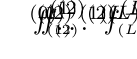
\begin{tikzpicture}
  % first two layers
  \node (in1)
  [inner sep=0]
  {\tikz \drawMessagesWithArrows{$\vz^{(0)}$}{ }{ }{\hNodeDistance};};
  \node (layer1)
  [anchor=south west, inner sep=0]
  at (in1.south east)
  {\tikz \drawModuleWithParams{$f^{(1)}_{\vtheta^{(1)}}$}{16}{$\vtheta^{(1)}$}{ }{ };};
  \node (out1)
  [inner sep=0, anchor=south west]
  at (layer1.south east)
  {\tikz \drawMessagesWithArrows{$\vz^{(1)}$}{ }{ }{\hNodeDistance};};
  \node (layer2)
  [inner sep=0pt, anchor=south west]
  at (out1.south east)
  {\tikz \drawModuleWithParams{$f^{(2)}_{\vtheta^{(2)}}$}{16}{$\vtheta^{(2)}$}{ }{ };};

  % dots with messages
  \node (in2)
  [inner sep=0, anchor=south west]
  at (layer2.south east)
  {\tikz \drawMessagesWithArrows{$\vz^{(2)}$}{ }{ }{\hNodeDistance};};
  \node (dots)
  [xshift=0.75ex, inner sep=0pt, anchor=west]
  at (in2.east)
  {$\dots$};

  \node (inLast)
  [xshift=0.75ex, inner sep=0pt, anchor=west]
  at (dots.east)
  {\tikz \drawMessagesWithArrows{$\vz^{(L-1)}$}{ }{ }{\hNodeDistance};};

  \node (layerLast)
  [anchor=south west, inner sep=0]
  at (inLast.south east)
  {\tikz \drawModuleWithParams{$f^{(L)}_{\vtheta^{(L)}}$}{16}{$\vtheta^{(L)}$}{ }{ };};
  \node (outLast)
  [inner sep=0, anchor=south west]
  at (layerLast.south east)
  {\tikz \drawMessagesWithArrows{$\vz^{(L)}$}{ }{ }{\hNodeDistance};};
\end{tikzpicture}

%%% Local Variables:
%%% mode: latex
%%% TeX-master: "../../thesis"
%%% End:
